%
% Niniejszy plik stanowi przykład formatowania pracy magisterskiej na
% Wydziale MIM UW.  Szkielet użytych poleceń można wykorzystywać do
% woli, np. formatujac wlasna prace.
%
% Zawartosc merytoryczna stanowi oryginalnosiagniecie
% naukowosciowe Marcina Wolinskiego.  Wszelkie prawa zastrzeżone.
%
% Copyright (c) 2001 by Marcin Woliński <M.Wolinski@gust.org.pl>
% Poprawki spowodowane zmianami przepisów - Marcin Szczuka, 1.10.2004
% Poprawki spowodowane zmianami przepisow i ujednolicenie 
% - Seweryn Karłowicz, 05.05.2006
% Dodanie wielu autorów i tłumaczenia na angielski - Kuba Pochrybniak, 29.11.2016

% dodaj opcję [licencjacka] dla pracy licencjackiej
% dodaj opcję [en] dla wersji angielskiej (mogą być obie: [licencjacka,en])
\documentclass[magisterska,en]{pracamgr}

\usepackage{algorithm}
\usepackage{algpseudocode}
\usepackage{amsfonts}
\usepackage{amsmath}
\usepackage{amssymb}
\usepackage{graphicx}
\usepackage{hyperref}
\usepackage{minted}
\usepackage{pgfplots}

\usetikzlibrary{intersections, pgfplots.fillbetween, trees}

\hypersetup{
    colorlinks,
    citecolor=black,
    filecolor=black,
    linkcolor=black,
    urlcolor=black
}

\newcommand\chartsize{0.94}

% Dane magistranta:
\autor{Grzegorz Nowakowski}{429576}

\title{NP-hard Metrics for Evaluating Participatory Budgeting Rules}
\titlepl{NP-trudne metryki do oceny reguł wyborczych dla budżetów partycypacyjnych}

\kierunek{Computer Science}

% informatyka - nie okreslamy zakresu (opcja zakomentowana)
% matematyka - zakres moze pozostac nieokreslony,
% a jesli ma byc okreslony dla pracy mgr,
% to przyjmuje jedna z wartosci:
% {metod matematycznych w finansach}
% {metod matematycznych w ubezpieczeniach}
% {matematyki stosowanej}
% {nauczania matematyki}
% Dla pracy licencjackiej mamy natomiast
% mozliwosc wpisania takiej wartosci zakresu:
% {Jednoczesnych Studiow Ekonomiczno--Matematycznych}

% \zakres{Tu wpisac, jesli trzeba, jedna z opcji podanych wyzej}

% Praca wykonana pod kierunkiem:
% (podać tytuł/stopień imię i nazwisko opiekuna
% Instytut
% ew. Wydział ew. Uczelnia (jeżeli nie MIM UW))
\opiekun{Prof. Piotr Skowron}

\date{June 2025}

%Dziedzina wg klasyfikacji Socrates-Erasmus:
\dziedzina{11.3 Informatics}

%Klasyfikacja tematyczna wedlug ACM (informatyka)
\klasyfikacja{
    D. Software\\
    F. Theory of Computation\\
    I. Computing Methodologies
  }

% Słowa kluczowe:
\keywords{Social Choice, Participatory Budgeting, Computational Complexity}

\begin{document}
\maketitle

\begin{abstract}

A participatory budgeting election is a tuple consisting of a set of voters, a set of candidates, a budget, a cost function that assigns a cost to each candidate, and a set of ballots cast by the voters regarding the candidates. An election rule is a function that returns an outcome for a given election instance; an outcome is a subset of candidates whose total cost does not exceed the given budget.

Various metrics are used to evaluate outcomes, and so election rules with respect to fairness and efficiency. In some cases, determining whether an outcome satisfies a specific criterion, such as being in the core, is NP-hard. This thesis aims to implement algorithms for verifying such NP-hard metrics, enabling computations for as large elections as possible. The metrics of particular interest are the core and Pareto optimality. We will also propose relaxations of these metrics to indicate the extent to which a given criterion is violated.

Our algorithms will be implemented in the Pabutools open-source library and tested on real data from Pabulib.
\end{abstract}

\tableofcontents
%\listoffigures
%\listoftables

\chapter*{Introduction}
\addcontentsline{toc}{chapter}{Introduction}

Social choice theory studies how collective decisions are made based on individual preferences. In particular, for a set of candidates and voters with their preferences over those candidates, it investigates how various voting rules influence outcomes and how desirable properties, such as efficiency, fairness, or stability, can be ensured.

One prominent area of application of social choice theory is participatory budgeting, where a community selects a subset of public projects to fund, subject to a budget constraint. Projects may have different costs, and each voter expresses their preferences over the available options. The preference model may be ranking-based, where each voter assigns a rank to every candidate, or approval-based, where the voters’ ranks are binary (0 or 1) --- indicating whether they approve a candidate or not. The challenge lies in aggregating these preferences in a way that respects both individual satisfaction and collective fairness.

In this context,  one efficiency notion could be the average satisfaction of voters with the funded projects, and one of the most important and widely researched fairness and stability properties is the core, which ensures there is no group of voters who could propose a different set of projects that would leave them all strictly better off, given that the size of the group is proportional to the cost of the proposed set of projects.

To distinguish between these two models, let us consider a few examples. In the first model, we fix a committee size $k$ and the goal is to select a committee of exactly $k$ members. Real-world examples include presidential elections, where $k=1$, or parliamentary elections, where $k=460$ (as in Poland). In participatory budgeting, on the other hand, we are given a budget $b$, and the goal is to select a subset of projects whose total cost does not exceed $b$. This is typically organized by cities or small towns that allocate funds to social projects, such as bike paths, new parks, gyms, or public infrastructure.

In recent years, participatory budgeting has received growing attention due to its real-world relevance and computational complexity. To support experimental research in this area, a Python-based toolkit called \texttt{Pabutools}\cite{1} has been developed. This library provides a comprehensive interface for defining elections, applying voting rules, and evaluating outcomes. All election data are fetched from \texttt{Pabulib}\cite{2}, a standardized repository of real and synthetic election instances. Results can also be explored interactively using the web-based API \texttt{Pabustats}~\cite{3}, which offers a user-friendly platform for experimenting with voting rules and visualizing their performance.

This thesis focuses on evaluating voting rules through the lens of two key theoretical properties: core and Pareto efficiency. These properties, referred to as metrics, provide formal guarantees of fairness and optimality. While their definitions are mathematically elegant, they pose significant computational challenges. In fact, both verifying and finding outcomes that satisfy these metrics is known to be NP-hard in general~\cite{4}~\cite{5}. From the perspective of computational complexity theory, NP-hard problems are those for which no polynomial-time algorithms are likely to exist. What is more, for core and Pareto efficiency, we cannot even verify in polynomial time whether a given solution satisfies the respective property. This computational barrier makes brute-force approaches impractical, even for elections of moderate size.

Participatory budgeting is not just a theoretical model --- it has a direct impact on real-world political decisions and community outcomes. Fairness criteria such as proportionality, core stability, and Pareto efficiency aim to ensure that minority groups are not discriminated and that no group of voters can unilaterally impose or block decisions. These properties help prevent both minority domination and the marginalization of significant number of the electorate. However, the large number of voters in practical elections and the computational complexity of satisfying such axioms pose significant challenges. Despite this, ensuring fairness and stability remains an essential goal. This thesis faces these challenges by exploring efficient algorithmic approaches to test and improve the compliance of voting rules with core and Pareto optimality properties.

To overcome these difficulties, we use integer linear programming (ILP) formulations, which allow us to encode the conditions of these problems in a format that modern optimization solvers can handle efficiently. Linear programming is a mathematical optimization technique that finds the maximum or minimum of a linear objective function subject to linear constraints. Integer linear programming is a special case where all variables must take integer values, making it a good fit for settings such as voting, where decisions are often binary.

As an example, consider a participatory budgeting scenario with two types of projects: type A and type B. Type A projects cost 2 units of budget and require 1 day of administrative effort, while type B projects cost 1 unit of budget and require 2 days of administrative effort. The city has a total budget of $b=100$ and can allocate at most 80 days of administrative effort. The goal is to maximize the total satisfaction of a citizen who assigns a utility of 40 to each type A project and 30 to each type B project. Let $x$ be the number of type A projects to be funded and $y$ the number of type B projects. We aim to maximize the satisfaction function $P=40x+30y$, subject to the constraints $2x+y\leq100$, $x+2y\leq80$, and $x,y\geq0$. These constraints are illustrated in Figure~\ref{ilp-example}:

\begin{figure}[h!]
    \centering
    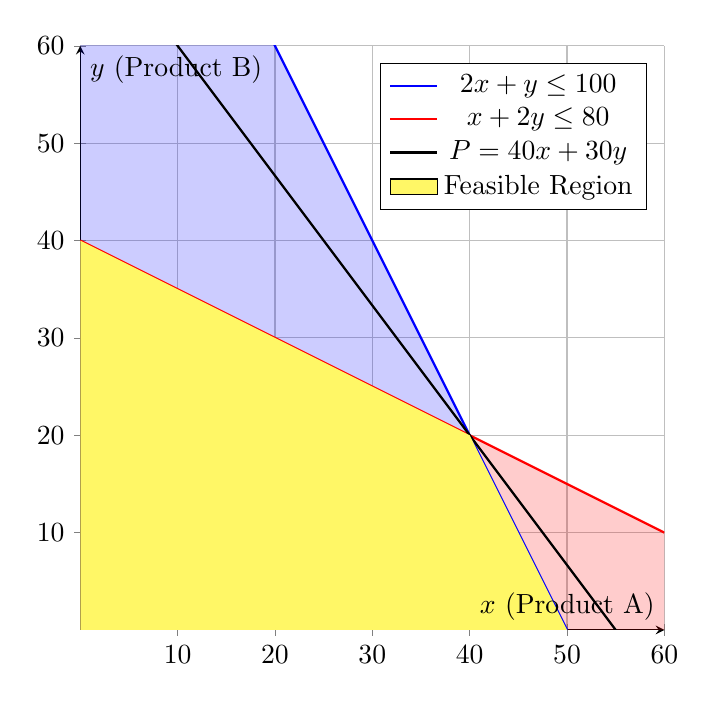
\begin{tikzpicture}
        \begin{axis}[
            width=9cm,
            height=9cm,
            axis lines=middle,
            xlabel={$x$ (Product A)},
            ylabel={$y$ (Product B)},
            xmin=0, xmax=60,
            ymin=0, ymax=60,
            grid=both,
            legend pos=north east,
            samples=100,
            domain=0:60
        ]
        
        % Plot constraints
        \addplot[domain=0:50, thick, blue] {100 - 2 * x};
        \addlegendentry{$2x + y \leq 100$}
        
        \addplot[domain=0:60, thick, red] {(80 - x) / 2};
        \addlegendentry{$x + 2y \leq 80$}
        
        \addplot[domain=0:60, thick, black] {(2200 - 40 * x) / 30};
        \addlegendentry{$P=40x+30y$}
        
        % Fill feasible region
        \addplot[
            fill=yellow!60,
            draw=none,
            area legend,
        ] coordinates {
            (0,0)
            (0,40)
            (40,20)
            (50,0)
            (0,0)
        };
        \addlegendentry{Feasible Region}
        
        \addplot[name path=A, domain=0:50, draw=none] {100 - 2*x};
        \path[name path=axis] (axis cs:0,0) -- (axis cs:50,0);
        \addplot [
            thick,
            color=blue,
            fill=blue,
            fill opacity=0.2,
        ] fill between[of=A and axis];
        
        \addplot[name path=B, domain=0:60, draw=none] {(80 - x)/2};
        \path[name path=axis2] (axis cs:0,0) -- (axis cs:60,0);
        \addplot [
            thick,
            color=red,
            fill=red,
            fill opacity=0.2,
        ] fill between[of=B and axis2];
        
        \end{axis}
    \end{tikzpicture}
    
    \caption{ILP example constraints presented on the coordinate system.}
    \label{ilp-example}
\end{figure}

The yellow region is the feasible region, meaning all points inside it satisfy the constraints. In general, this is an example of a linear programming problem, but in our example we cannot fund half of a project, thus this is a particularly integer linear programming problem: both $x$ and $y$ must be integers. Rewriting the objective function as $y=(P-40x)/30$ shows that it has a fixed slope. We need to choose $P$ such that there is only one intersection point with the yellow region --- the only maximal solution. This point is $(40,20)$, giving the maximum utility of $P=2200$.

To solve such problems efficiently, various solvers have been developed. Modern solvers such as Gurobi~\cite{6} can handle large instances in practice, although solving time can still be a bottleneck. One of the main goals of this thesis is to investigate and implement techniques that further improve solver performance in this setting.

Finally, three well-known voting rules are experimentally benchmarked: Method of Equal Shares, Bounded Overspending, and Utilitarian Greedy. Each rule is evaluated against the two NP-hard metrics (core and Pareto efficiency), and the results are compared both in terms of theoretical expectations and empirical performance. Through the use of optimized solvers and real-life datasets, this thesis provides insights into the trade-offs between fairness, efficiency, and computational tractability in participatory budgeting.

The thesis is organized into five chapters. Chapter~\ref{preliminaries} introduces the theoretical model of participatory budgeting, the voting rules, and the evaluation properties studied throughout this work. It also discusses integer linear programming and how modern solvers address such problems. Chapter~\ref{algorithms-and-heuristics} presents ILP formulations of core and Pareto efficiency and explores optimization ideas for speeding up the computation. These ideas are benchmarked in Chapter~\ref{algorithms-analysis}, which presents and analyses their performance. Chapter~\ref{algorithms-applications} evaluates the voting rules in terms of their satisfaction of the evaluation properties and compares the outcomes with randomized budget allocation. All findings are summarized in Chapter~\ref{summary}.

All source code, including the ILP models, voting rules, and utility functions described in this work, is publicly available on GitHub~\cite{7}~\cite{8}.

\chapter{Preliminaries}
\label{preliminaries}

This chapter expands on the introductory concepts by providing formal definitions and theoretical formulations. It also gives an overview of Gurobi’s heuristics and its methods for solving linear programming and integer linear programming problems.

\section{Participatory Budgeting Model}

An election in the PB model is defined as a tuple $E=(N, C, b, cost, \{A_i\}_{i\in N})$, where
\begin{itemize}
    \item $N$ is a set of voters.
    \item $C$ is a set of candidates (or projects).
    \item $b\in\mathbb{N}$ is the available budget.
    \item $cost:C\to\mathbb{N}$ is a function that assigns a cost to each candidate. Throughout this thesis, we use the notation $cost(T)=\sum_{p\in T}cost(p)$ for any subset $T\subseteq C$.
    \item $A_i$ is the ballot of the $i$-th voter, i.e. the set of projects that voter $i$ approves.
\end{itemize}

A subset of candidates $W\subseteq C$ is called feasible if its total cost does not exceed the budget, that is, $cost(W)\leq b$. The goal of participatory budgeting is to select a feasible outcome based on the voters' preferences.

In this thesis, we assume the model of cost utilities, where the utility of voter $i$ for a subset $T\subseteq C$ is defined as $u_i(T)=\sum_{p\in T\cap A_i} cost(p)$. In other words, it is the sum of the costs of the approved projects that are included in the outcome.

\section{Voting Rules}

To determine the final outcome, we apply a voting rule, which is a function $\mathcal{R}$ that, given an election $E$, returns a feasible outcome $W=\mathcal{R}(E)$. Numerous voting rules exist; in this thesis, we focus on three of them, described below.

\subsection{Greedy Utilitarian Welfare}

The first rule discussed in this thesis is the Greedy Utilitarian Welfare method. Its goal is to maximize the total utility of voters, that is, $\sum_{i\in N}u_i(W)$. While this problem is computationally hard in general, the greedy algorithm produces the outcome that is optimal up to one project. Formally, for the outcome $W$, there exists a project $p\notin W$ such that
$$
\sum_{i\in N}u_i(W\cup\{p\})\geq \max_{W':cost(W')\leq b}\sum_{i\in N}u_i(W').
$$

The algorithm proceeds as follows: start with an empty outcome $W=\emptyset$, and add projects in a loop until no projects remain. In each iteration, select the project $p$ that maximizes the ratio
$$
\sum_{i\in N}\frac{u_i(p)}{cost(p)}.
$$
If there is sufficient budget remaining for project $p$, add it to the outcome; otherwise, discard it from further consideration.

Since we assume cost utilities of the voters, this rule effectively selects projects in descending order of the number of approvals.

\subsection{Method of Equal Shares}

The second rule is the Method of Equal Shares, introduced in recent work by Peters and Skowron~\cite{9}.

Each voter initially receives an equal fraction of the budget, i.e., $b_i=\frac{b}{|N|}$. Starting with an empty outcome $W=\emptyset$, the candidates are sequentially added to $W$. To add a candidate $c$ to $W$, the voters must collectively pay its cost. For each selected candidate $c\in W$, let $p_i(c)$ denote the amount that voter $i$ contributes to $c$'s cost. We require
$$
\sum_{i\in N}p_i(c)=cost(c).
$$
Let $p_i(W)=\sum_{c\in W}p_i(c)\leq\frac{b}{|N|}$ be the total amount that the voter $i$ has spent so far. Then the remaining budget of the voter $i$ is $b_i=\frac{b}{|N|}-p_i(W)$. For a given $\rho>0$, a candidate $c\in W$ is called $\rho$-affordable if
$$
\sum_{i\in N}\min(b_i, \rho\cdot u_i(c)) = cost(c).
$$
If no candidate is $\rho$-affordable for any $\rho$, the rule terminates and returns $W$. Otherwise, it selects a candidate $c$ that is $\rho$-affordable for the smallest possible value of $\rho$. The individual payments are then defined by
$$
p_i(c) = \min(b_i, \rho\cdot u_i(c)).
$$

The Method of Equal Shares satisfies strong proportionality guarantees but often produces non-exhaustive outcomes. To address this issue, the method can be modified by increasing each voter's initial budget by 1 (or another fixed value) and rerunning the procedure. However, this approach does not guarantee an exhaustive outcome. To improve this further, the method can be extended by applying Greedy Utilitarian Welfare as a completion step after the initial Equal Shares process has finished.

For further reading, including real-world applications of MES, additional examples, and empirical data, visit the official Equal Shares website~\cite{10}.

\subsection{Bounded Overspending}

In a recent paper, Papasotiropoulos et al.~\cite{11} proposed a variant of the Method of Equal Shares, called Equal Shares with Bounded Overspending. In this model, voters are allowed to spend more than their initial budget $b_i$, under certain conditions.

Specifically, voters may buy an $\alpha$-fraction of a project, receiving the corresponding fraction of utility, while still being required to cover the full cost of the project. Formally, for $\alpha\in(0,1]$ and $\rho>0$, we say that a project $c$ is {$(\alpha,\rho)$-affordable} if:
$$
\sum_{i\in N}\min(b_i, \alpha\cdot\rho\cdot u_i(c)) = \alpha\cdot cost(c).
$$

The algorithm closely follows the basic Equal Shares procedure. Each voter starts with an initial budget $b_i=\frac{b}{|N|}$, and the initial outcome is empty; $W = \emptyset$. In each iteration, the rule selects a project that is $(\alpha,\rho)$-affordable for the smallest possible value of $\frac{\rho}{\alpha}$. The payment of voter $i$ for the project $c$ is defined as:
$$
p_i(c) = \min(b_i, \rho\cdot u_i(c)).
$$
If no project is $(\alpha,\rho)$-affordable for any $\alpha$ and $\rho$, the rule terminates and returns $W$.

\section{Axiomatic Properties}

Given the multitude of voting rules, we would like to assess which ones perform better. Although it is not possible to answer this question in absolute terms, we can evaluate the rules in terms of efficiency, fairness, and stability. For this purpose, various axiomatic properties have been proposed. The most relevant ones for this thesis are introduced in this section.

\subsection{Core}

One of the most important notions in the domains of fairness and stability is the core, first formalized by Aziz et al.~\cite{12} For an election instance $E=(N, C, b, cost, \{A_i\}_{i\in N})$, an outcome $W$ is in the core, if for every subset of voters $S\subseteq N$ and every subset of projects $T\subseteq C$ satisfying
$$
\frac{|S|}{|N|} \geq \frac{cost(T)}{b}
$$
there exists at least one voter $i\in S$ such that $u_i(W)\geq u_i(T)$.

In other words, no group of voters $S$ should be able to propose an alternative set of candidates $T$ that satisfies a proportionality condition (i.e., the group size relative to the electorate is at least the proportion of the budget required by $T$), and in which every voter in $S$ strictly prefers $T$ over the selected outcome $W$.

Being one of the most interesting and important properties, core is widely researched in recent works by Fain et al.~\cite{4}, Munagala et al.~\cite{13},~\cite{14}. In addition, it is coNP-hard to decide whether a given outcome is in the core~\cite{15}. Since we would like to be able to answer this question in finite time, many approximations of the core were proposed~\cite{13}~\cite{16}.

However, it is unknown whether there exists a voting rule that always produces an outcome in the core, i.e. for every election instance $E$, the outcome $W=\mathcal{R}(E)$ is in the core. Similarly, it is not known whether the core is always non-empty --- that is, whether there exist elections for which no outcome $W$ is in the core. These open questions apply specifically to approval-based committee elections. In contrast, for not approval-based committee model, counterexamples are already known; one such example can be found in the work of D. Peters et al.~\cite{17}, but in the PB model with cost-utilities, the core might be empty.

\subsection{Pareto Optimality}

The second property called Pareto optimality, or Pareto efficiency, has its roots in economics, but also applies to engineering, biology, and social choice theory. In general, it demands that there is no improvement, such that it leaves one person with a strictly higher utility, without leaving anyone else with lower utility. For the purpose of this thesis, we assume the definition proposed by Lackner and Skowron~\cite{18}.

More formally, an outcome $W_1$ dominates an outcome $W_2$ if every voter is at least as satisfied with $W_1$ as with $W_2$, and at least one voter strictly prefers $W_1$ over $W_2$. An outcome $W$ is called Pareto optimal if it is not dominated by any other feasible subset of projects.

This property is also computationally difficult. Aziz et al.~\cite{5} showed that it is coNP-complete to verify whether an outcome $W$ satisfies Pareto efficiency.

\section{Integer Linear Programming}

Linear programming is a method for solving mathematical optimization problems. Typically, we aim to find a vector $x\in\mathbb{R}^n$ that satisfies a set of linear constraints, expressed as $Ax\leq b$ for some matrix $A\in\mathbb{R}^{m,n}$ and vector $b\in\mathbb{R}^m$. The goal is to maximize or minimize a linear objective function of the form $f(x)=c^Tx$, where $c\in\mathbb{R}^n$. These constraints define a feasible region over which the optimal solution is sought. A subdomain of linear programming is integer linear programming (ILP), where all the variables must take integer values. It is worth mentioning that ILP problems are NP-hard to solve, in contrast to general LP problems, which can be solved in polynomial time.

There are several algorithms used to solve such problems. One of the most well-known and widely applied is the simplex method. The core idea of this method is to find a basic feasible solution (a vertex of the feasible region), and then iteratively move along the edges of the polytope to improve the objective value until an optimum is reached.

When it comes to solving integer programming problems, the branch and bound technique is one of the fundamental approaches. The main idea is to explore subsets of the feasible region by creating a search tree. Each node represents a subproblem with additional constraints --- restricting the value of a selected variable, such as fixing it to an integer or tightening its bounds. Bounding techniques are used to cut parts of the tree that cannot lead to better solutions.

A simple example of branch and bound in action is a PB instance with budget $b=50$, only one voter, and three projects with costs $cost(p_1)=10$, $cost(p_2)=20$, and $cost(p_3)=30$. The utilities of the voter on these projects are $u(p_1)=60$, $u(p_2)=100$, and $u(p_3)=120$. The ILP for this example is represented with three binary variables $x_1,x_2,x_3\in\{0,1\}$, a budget constraint $10x_1+20x_2+30x_3\leq50$, and the objective function to maximize $60x_1+100x_2+120x_3$.

First, we relax the integrality constraint and solve the linear relaxation with $x_i\in[0,1]$. The optimal relaxed solution is $x_1=x_2=1$, $x_3=\frac{2}{3}$, with a total profit of $60+100+80=240$. Since $x_3$ is fractional, we need to branch. The solver considers two subproblems: one with $x_3=0$ and another with $x_3=1$. Solving these subproblems eventually yields the optimal integer solution: $x_1=0$, $x_2=x_3=1$, with a total profit of $220$. The branch-and-bound tree is illustrated in Figure~\ref{branch-and-bound-tree}.

\begin{figure}[h!]
    \centering
    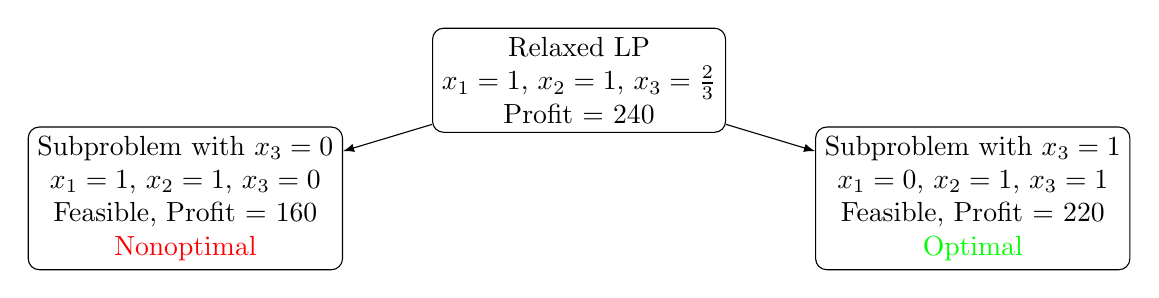
\begin{tikzpicture}[
        level 1/.style={sibling distance=10cm},
        level 2/.style={sibling distance=3cm},
        edge from parent/.style={draw, -latex},
        every node/.style={draw, rounded corners, align=center, minimum width=2.5cm}
    ]
        \node {Relaxed LP\\$x_1=1$, $x_2=1$, $x_3=\frac{2}{3}$\\Profit = 240}
            child {node {Subproblem with $x_3 = 0$\\$x_1=1$, $x_2=1$, $x_3=0$\\Feasible, Profit = 160\\\textcolor{red}{Nonoptimal}}}
            child {node {Subproblem with $x_3 = 1$\\$x_1=0$, $x_2=1$, $x_3=1$\\Feasible, Profit = 220\\\textcolor{green}{Optimal}}};
    \end{tikzpicture}

    \caption{The branch-and-bound tree for the exemplary problem.}
    \label{branch-and-bound-tree}
\end{figure}

Generally, branch and bound technique is not a brute-force approach. During the branching step, the algorithm selects a non-integer variable from the current LP-relaxed solution and creates two subproblems, by bounding this variable: to be less than or equal to the nearest smaller integer (first branch), and to be greater than or equal to the nearest larger integer (second branch). In the bounding step, the algorithm solves the LP relaxation of each subproblem and compares the solution's objective value with the best known feasible integer solution. If a relaxed subproblem yields a smaller profit than the current best, it is cut from the further consideration, since it cannot lead to a better solution.

Fortunately, such algorithms are not needed to be manually implemented as powerful solvers are available that handle LP and ILP problems efficiently. One such solver used in this thesis is Gurobi, which will be discussed in the following section.

\section{Gurobi}

Gurobi Optimizer is a commercial solver developed by Gurobi Optimization, LLC, designed to solve a wide range of mathematical optimization problems. It is recognized for its high performance and efficiency, including a variety of advanced techniques, particularly for linear programming. Gurobi is widely used across industries, including finance, logistics, and research, to find optimal solutions for large-scale and complex problems.

In the case of linear programming problems, Gurobi primarily uses the simplex method~\cite{19} to determine a basic feasible solution and iteratively improve the objective value. For mixed-integer programming, it applies sophisticated branch-and-bound and cutting-plane techniques, enhanced by heuristics and presolve strategies.

Gurobi offers user-friendly APIs in several popular programming languages, including C++, Java, and Python. Given that the Pabutools framework, used extensively throughout this thesis, is implemented in Python, the corresponding Python interface, \texttt{gurobipy}, was used.

As discussed later in the thesis, NP-hard axiomatic properties, such as core and Pareto optimality, are computed via their corresponding integer linear programming problems. To ensure that these computations are as efficient as possible, Gurobi, with its powerful optimization capabilities, was chosen as the solver of choice.

\chapter{Algorithms and Heuristics}
\label{algorithms-and-heuristics}

This chapter presents the main axiomatic properties as ILP formulations and describes key optimization techniques evaluated later in this thesis, which may potentially speed up the ILP solving process.

\section{Core Verification}

The core property in approval-based participatory budgeting is known to be NP-hard to determine whether a core allocation exists, and coNP-hard to verify if a given allocation lies in the core. This implies not only that finding an outcome satisfying this property is computationally difficult, but also that verifying whether a given solution lies in the core is itself a hard problem. In particular, checking all possible combinations of voters and projects under the definition of a blocking coalition is infeasible, even for relatively small instances.

While rules that are likely to yield outcomes in core will be discussed later in this thesis, an important question arises: how can such outcomes be verified in finite time? Here, integer linear programming (ILP) provides a practical solution.

\subsection{ILP implementation}

The ILP program presented in Figure~\ref{core-ILP} is designed to search for a blocking coalition, if one exists. It introduces two types of binary variables: $x_c$ indicates whether project $c$ is included in the proposed set of projects $T$, and $y_i$ indicates whether voter $i$ is included in the proposed set of voters $V$. A blocking coalition must be non-empty, as ensured by constraint (\thechapter.1) and must satisfy the proportionality condition from the core definition, which is formulated in (\thechapter.2). This constraint also implicitly guarantees that the selected projects do not exceed the budget, making an explicit budget constraint unnecessary. Finally, constraint (\thechapter.3) ensures that each voter in the blocking set $V$ is strictly more satisfied with the proposed set $T$ than with the outcome $W$.

Notably, the program has no objective function --- its sole purpose is to determine feasibility. If there is a solution that satisfies all the constraints, it serves as a certificate that the outcome $W$ violates the core.

\begin{figure}[h!]
$$
\boxed{
\renewcommand{\arraystretch}{1.3}
\begin{array}{rlrr}
\textbf{maximize}    & 0 & \\
\textbf{subject to:} & x_c\in\{0,1\} & \mbox{for } c\in C & \\
                     & y_i\in\{0,1\} & \mbox{for } i\in N & \\
                     & \sum_{i\in N}y_i\geq 1 & & \text{(\thechapter.1)} \\
                     & \sum_{c\in C}x_c\cdot cost(x_c)\cdot|N|\leq\sum_{i\in N}y_i\cdot b & & \text{(\thechapter.2)} \\
                     & \sum_{c\in A_i}x_c\cdot cost(x_c)\geq y_i\cdot(u_i(W)+1) & \mbox{for } i\in N & \text{(\thechapter.3)}
\end{array}
}
$$
\caption{An ILP for verifying the core property.}
\label{core-ILP}
\end{figure}

\subsection{Relaxations}

A natural idea to improve the solver's performance is to relax the variable types from integers to continuous values. Fractional solutions form a superset of integer ones and are typically much faster to compute. Therefore, if the relaxed program does not find a solution, we can safely conclude that no integer solution exists either, and hence no blocking coalition can be found.

We may apply this relaxation selectively --- to voters, projects, or both. If all of these relaxed programs admit a solution, we cannot draw a definitive conclusion. However, if one of them fails to find one, we can conclude that no integer solution exists either --- meaning that, for the given election instance, the outcome satisfies the core property.

Consider Example~\ref{ilp-example} from the introduction. It involved two variables $x,y\geq0$ and constraints $2x+y\leq100$ and $x+2y\leq80$, with an objective function $P=40x+30y$ to maximize. Now, imagine we add a third constraint: $x+y\geq70$. The updated feasible region is shown in Figure~\ref{ilp-example-2}.

\begin{figure}[h!]
    \centering
    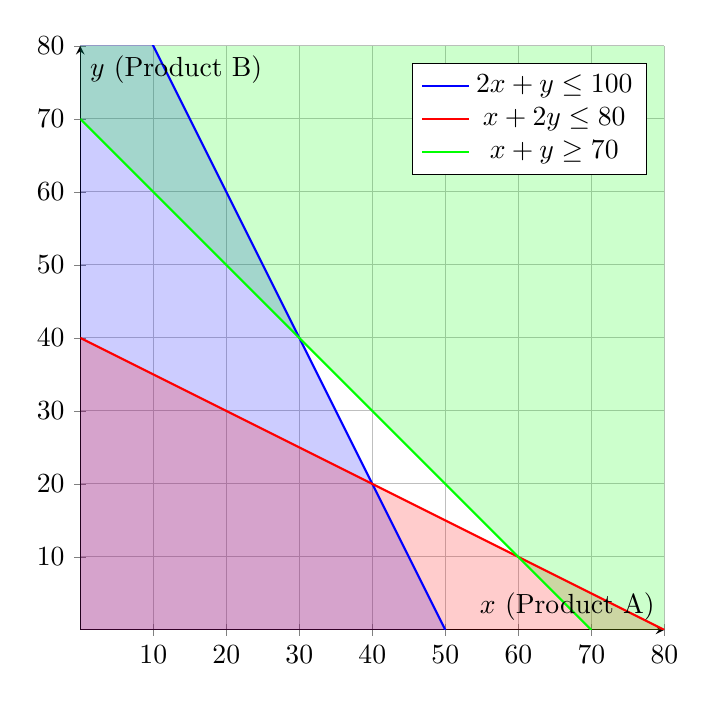
\begin{tikzpicture}
        \begin{axis}[
            width=9cm,
            height=9cm,
            axis lines=middle,
            xlabel={$x$ (Product A)},
            ylabel={$y$ (Product B)},
            xmin=0, xmax=80,
            ymin=0, ymax=80,
            grid=both,
            legend pos=north east,
            samples=100,
            domain=0:80,
        ]
        
        % Plot constraints
        \addplot[domain=0:50, thick, blue] {100 - 2 * x};
        \addlegendentry{$2x + y \leq 100$}
        
        \addplot[domain=0:80, thick, red] {(80 - x) / 2};
        \addlegendentry{$x + 2y \leq 80$}
    
        \addplot[domain=0:70, thick, green] {-x + 70};
        \addlegendentry{$x+y\geq70$}


        % Fill regions
        \addplot[name path=A, domain=0:50, draw=none] {100 - 2*x};
        \path[name path=axis] (axis cs:0,0) -- (axis cs:50,0);
        \addplot [
            thick,
            color=blue,
            fill=blue,
            fill opacity=0.2,
        ] fill between[of=A and axis];

        \addplot[name path=B, domain=0:60, draw=none] {(80 - x)/2};
        \path[name path=axis2] (axis cs:0,0) -- (axis cs:80,0);
        \addplot [
            thick,
            color=red,
            fill=red,
            fill opacity=0.2,
        ] fill between[of=B and axis2];

        \addplot[name path=C, domain=0:80, draw=none] {-x + 70};
        \path[name path=top] (axis cs:0,80) -- (axis cs:80,80);
        \addplot [
            thick,
            color=green,
            fill=green,
            fill opacity=0.2,
        ] fill between[of=top and C];
        
        \end{axis}
    \end{tikzpicture}

    \caption{Updated ILP example with an additional constraint, shown graphically.}
    \label{ilp-example-2}
\end{figure}

As seen in the figure, there is no feasible region where all three shaded areas intersect. This means the problem has no solution --- neither integer nor fractional. In practice, solving the relaxed version of a problem (i.e., allowing non-integer variables) is often faster and can immediately reveal such infeasibility, especially in large-scale ILPs. This illustrates the core idea behind using LP relaxations.

\subsection{Branching Priority}

Gurobi allows for the assignment of attributes to model variables to influence the solving process. One such attribute is \texttt{BranchPriority}, which affects the variable selection order during the \textit{branch and bound} procedure. Variables with higher priority values are branched on earlier.

In the core-verifying ILP, this attribute can be used for both project and voter variables. For projects, one possible heuristic is to prioritize those with a high approval-to-cost ratio, as expensive or weakly approved projects are unlikely to appear in a blocking coalition. For voters, the idea is to prioritize those with lower current satisfaction, as it is easier to improve their utility with a different set of projects.

Consider an ILP with three binary variables $x_1,x_2,x_3$ and a single constraint $x_1+x_2+x_3\leq1$. Assume that the solver considers variables in lexicographical order by default. If we instead set the \texttt{BranchPriority} attributes of these variables to 3, 10, and 5 respectively, then the branching order will change, and the solver will prioritize branching on $x_2$ first. Figure~\ref{branching-example} shows sketches of the resulting branch-and-bound trees: the default one on the left, and the one with custom branching priorities on the right.

\begin{figure}[h!]
    \begin{minipage}[c]{0.5\textwidth}
    \begin{tikzpicture}
        \begin{scope}[every node/.style={circle, draw=none, minimum size=10mm, inner sep=2pt}]
            \node (1) at (0, 0) {$x_1$};
            \node (2) at (-2, -2) {$x_2$};
            \node (3) at (2, -2) {$x_2$};
            \node (4) at (-3, -4) {$x_3=0$};
            \node (5) at (-1, -4) {$x_3=1$};
            \node (6) at (1, -4) {$x_3=0$};
            \node (7) at (3, -4) {$x_3=1$};
        \end{scope}
        
        \draw[->] (1) -- (2) node[midway, above left] {$0$};
        \draw[->] (1) -- (3) node[midway, above right] {$1$};
        \draw[->] (2) -- (4) node[midway, left] {$0$};
        \draw[->] (2) -- (5) node[midway, right] {$1$};
        \draw[->] (3) -- (6) node[midway, left] {$0$};
        \draw[->] (3) -- (7) node[midway, right] {$1$};
    \end{tikzpicture}
    \end{minipage}
    \begin{minipage}[c]{0.5\textwidth}
    \begin{tikzpicture}
        \begin{scope}[every node/.style={circle, draw=none, minimum size=10mm, inner sep=2pt}]
            \node (1) at (0, 0) {$x_2$};
            \node (2) at (-2, -2) {$x_3$};
            \node (3) at (2, -2) {$x_3$};
            \node (4) at (-3, -4) {$x_1=0$};
            \node (5) at (-1, -4) {$x_1=1$};
            \node (6) at (1, -4) {$x_1=0$};
            \node (7) at (3, -4) {$x_1=1$};
        \end{scope}
        
        \draw[->] (1) -- (2) node[midway, above left] {$0$};
        \draw[->] (1) -- (3) node[midway, above right] {$1$};
        \draw[->] (2) -- (4) node[midway, left] {$0$};
        \draw[->] (2) -- (5) node[midway, right] {$1$};
        \draw[->] (3) -- (6) node[midway, left] {$0$};
        \draw[->] (3) -- (7) node[midway, right] {$1$};
    \end{tikzpicture}
    \end{minipage}
    
    \caption{Comparison of two branch-and-bound trees an ILP solver might generate: without any branching priorities (left), and with \texttt{BranchPriority} attributes applied (right).}
    \label{branching-example}
\end{figure}

\subsection{Variable Start and Hint Values}

Two more useful attributes in Gurobi are \texttt{Start} and \texttt{VarHintVal}. Although they seem similar, they serve different purposes.

The \texttt{Start} attribute helps the solver to quickly identify a feasible solution. By providing a partially filled starting vector, the solver attempts to complete it and use it as an initial feasible point.

The \texttt{VarHintVal} attribute serves a suggestion or guess about the likely value of a variable. These hints guide the solver's internal heuristics and branching logic. Good hints can significantly speed up the solving process, while poor hints generally do not degrade performance. Additionally, hints can be paired with the \texttt{VarHintPri} attribute to indicate the user's confidence in each guess.

In the context of core-verifying, this technique can be used to suggest that voters with current satisfaction equal to zero are strong candidates for forming a blocking coalition, since adding just one of their approved projects improves their utility.

Consider a PB instance with budget $b=5$, a single voter, and three projects with costs $cost(p_1)=4$, $cost(p_2)=2$, and $cost(p_3)=3$. The voter's utilities for these projects are $u(p_1)=10$, $u(p_2)=6$, and $u(p_3)=8$. The ILP's objective is to maximize the function $10x_1+6x_2+8x_3$, subject to the constraint $4x_1+2x_2+3x_3\leq5$. If the solver were to prioritize variables in lexicographical order by default, it would consider $x_1$ first, leading to suboptimal branching, as this item consumes most of the capacity.

To guide the solver toward a better starting point or a promising region of the search space, we can compute the utility-to-cost ratios: 2.5 for $x_1$, 3 for $x_2$, and approximately 2.67 for $x_3$. Based on these, we can suggest that the solver first considers $x_2$ and $x_3$, which together yield a feasible solution of utility 14 and total cost 5.

This suggestion can be implemented using the \texttt{Start} attribute (providing a feasible initial solution), or the \texttt{VarHintVal} attribute (guiding the solver's branching decisions). While the solver still needs to verify optimality, in the case of core-verifying ILP, we are only interested in feasibility. Hence, such hinting mechanisms can be particularly effective in reducing runtime.

\subsection{Removing maximal satisfied voters}

Before the solving process, if a voter has already achieved the maximum possible satisfaction with the given outcome, they can be safely excluded from consideration. This is done by adding the constraint $y_i=0$, which effectively removes the corresponding variable from the search space in the presolve step. Since a blocking coalition requires strictly increasing utility of all its members, including fully satisfied voters would violate this requirement.

Such constraints eliminate corresponding variables from the branching tree, reducing its complexity. This simplification often leads to significant performance improvements when searching for feasible solutions.

\section{Pareto Optimality Verification}

Verifying Pareto efficiency in the PB model is computationally challenging as well. It requires checking all possible subsets of projects and evaluating their effects on each voter's utility --- an infeasible task for large instances.

To overcome this, we again resort to ILP, which provides a tractable approach to test Pareto optimality in practice.

\subsection{ILP implementation}

The ILP formulation for checking Pareto optimality is shown in Figure~\ref{pareto-ILP}. As with core checking, this program introduces two types of binary variables: $x_c$ indicates whether project $c$ is included in an alternative outcome $W'$ that may dominate the current outcome $W$, and $y_i$ identifies whether voter $i$ is strictly better off under $W'$. Since we need just one voter with strictly higher utility with $W'$, the (\thechapter.5) equation is formulated. We also cannot exceed the budget, which is guaranteed by (\thechapter.4). The last condition that must be met to make $W_1$ a dominant set over $W$, is to make one voter happier without lowering the utility of the others, which is formulated in (\thechapter.6).

As in the core-verifying ILP, we do not have to optimize any objective function, because satisfying all the constraints is equivalent to finding a set of projects that dominates $W$, and so violates the Pareto efficiency.

\begin{figure}[h!]
$$
\boxed{
\renewcommand{\arraystretch}{1.3}
\begin{array}{rlrr}
\textbf{maximize}    & 0 & \\
\textbf{subject to:} & x_c\in\{0,1\} & \mbox{for } c\in C & \\
                     & y_i\in\{0,1\} & \mbox{for } i\in N & \\
                     & \sum_{c\in C}x_c\cdot cost(x_c)\leq b & & \text{(\thechapter.4)} \\
                     & \sum_{i\in N}y_i=1 & & \text{(\thechapter.5)} \\
                     & \sum_{c\in A_i}x_c\cdot cost(x_c)\geq u_i(W)+y_i & \mbox{for } i\in N & \text{(\thechapter.6)}
\end{array}
}
$$
\caption{An ILP for verifying the Pareto optimality.}
\label{pareto-ILP}
\end{figure}

\subsection{Essential Projects}

To accelerate the ILP solving process, certain preprocessing steps can be applied. One useful observation concerns voters who have already achieved their maximum possible utility with the outcome $W$. This occurs when all projects from a voter's approval ballot $A_i$ are included in $W$.

In such cases, any alternative outcome $W_1$ that dominates $W$ must also include all these projects. Otherwise, the voter would strictly lose utility, violating the dominance condition of Pareto optimality.

This insight allows us to fix the corresponding decision variables in advance. Specifically, for each project $c\in A_i$ where $i$ is such a fully satisfied voter, we can add the constraint $x_c=1$ to the ILP. This reduces the solution space and can lead to significant performance improvements in practice.

\chapter{Algorithms Analysis}
\label{algorithms-analysis}

This chapter presents both time and quality analyses of the previously discussed methods. Since all techniques have already been thoroughly introduced, the following sections focus exclusively on performance improvements of the solver and the verification of proof-of-concept ideas.

All charts are divided into five groups: \texttt{all\_10}, \texttt{all\_30}, \texttt{all\_50}, \texttt{all\_100}, and \texttt{all}. These correspond to election instances categorized by the number of projects: fewer than 10, from 10 to 30, from 30 to 50, from 50 to 100, and over 100, respectively.

The programs were executed 10 times on each instance to reduce statistical noise, avoid anomalies, and produce more reliable average values. For clarity, the execution times were then sorted in ascending order to illustrate how quickly a given percentage of election instances could be solved.

\section{Vanilla ILPs}

First, we evaluate how the vanilla ILP algorithms from Figures~\ref{core-ILP} and~\ref{pareto-ILP} perform on the Pabulib instances, with respect to the three voting rules introduced earlier.

Several interesting observations emerge from these results. Most notably, checking Pareto optimality is significantly faster than verifying the core. The primary reason is structural: core-verifying requires variables for both projects and voters, with no fixed bounds on the size of potential blocking coalitions. In contrast, Pareto checking also uses voter variables, but only one of them is set to one, greatly simplifying the computation.

Another notable point is that verifying the core takes considerably longer for the Method of Equal Shares than for the Utilitarian Greedy rule (see Figures~\ref{vanilla-mes-core} and~\ref{vanilla-greedy-core}). This is because MES typically produces core-satisfying outcomes, whereas UG satisfies the core in only about half of the cases (detailed results are discussed in the next chapter). If no blocking coalition exists, the solver must exhaustively explore the entire branch-and-cut tree to verify core membership. In contrast, when a blocking coalition is found early, the solver can terminate quickly.

It is worth mentioning that a 30-minute timeout was set, as in some cases the ILP solver runs for a very long time. To prevent such outliers from distorting the analysis, these instances are excluded from the average computation, but their occurrence is indicated in the charts.

The following sections examine how various improvement strategies and relaxations affect the execution time of the ILP programs. Namely, we explore how future charts differ from the ones shown below. The analysis continues to focus on MES and UG, as their underlying principles differ significantly, as do their performances with respect to the evaluated metrics.

\begin{figure}[h!]
    \centering
    \includegraphics[width=\chartsize\linewidth]{outputs/NoOptimizations/mes-core.png}
    \caption{Execution time of vanilla core-verifying ILP on Method of Equal Shares outcomes.}
    \label{vanilla-mes-core}
\end{figure}

\begin{figure}[h!]
    \centering
    \includegraphics[width=\chartsize\linewidth]{outputs/NoOptimizations/mes-po.png}
    \caption{Execution time of vanilla PO-verifying ILP on Method of Equal Shares outcomes.}
    \label{vanilla-mes-po}
\end{figure}

\begin{figure}[h!]
    \centering
    \includegraphics[width=\chartsize\linewidth]{outputs/NoOptimizations/greedy-core.png}
    \caption{Execution time of vanilla core-verifying ILP on Utilitarian Greedy outcomes.}
    \label{vanilla-greedy-core}
\end{figure}

\begin{figure}[h!]
    \centering
    \includegraphics[width=\chartsize\linewidth]{outputs/NoOptimizations/greedy-po.png}
    \caption{Execution time of vanilla PO-verifying ILP on Utilitarian Greedy outcomes.}
    \label{vanilla-greedy-po}
\end{figure}

\section{Relaxations}

As discussed previously, if a relaxed linear program fails to find a feasible solution, it guarantees that no solution exists for the corresponding integer linear program either. This section analyses how efficiently we can determine the non-existence of a blocking coalition using relaxations, and evaluates both the runtime and the effectiveness of this approach.

The analysis is divided into two parts: one for the Method of Equal Shares and one for Utilitarian Greedy. The reason for this separation is the significant difference in the frequency with which these rules produce the core outcomes. For MES, we focus solely on checking core satisfaction. For UG, we also assess how often relaxations help identify a blocking coalition.

Starting with MES, we observe that the total execution time for all three types of relaxations, (i) projects and voters, (ii) only projects, and (iii) only voters, is lower than the runtime of the vanilla algorithm. However, a definitive answer was obtained in only 28\% of the cases. As shown in Figure~\ref{relaxations-mes}, all three relaxations agreed in only 8 instances. Individually, the project-only and voter-only relaxations provided answers in 70 and 96 instances, respectively. Notably, their results were mutually exclusive: there were no cases where both relaxations confirmed core satisfaction for the same instance.

\begin{figure}[h!]
    \centering
    \includegraphics[width=\chartsize\linewidth]{outputs/Relaxations/mes.png}
    \caption{Combined execution times of core-verifying ILP with projects, voters, and both relaxations on Method of Equal Shares outcomes.}
    \label{relaxations-mes-time}
\end{figure}

\begin{figure}[h!]
    \begin{minipage}[c]{0.5\textwidth}
    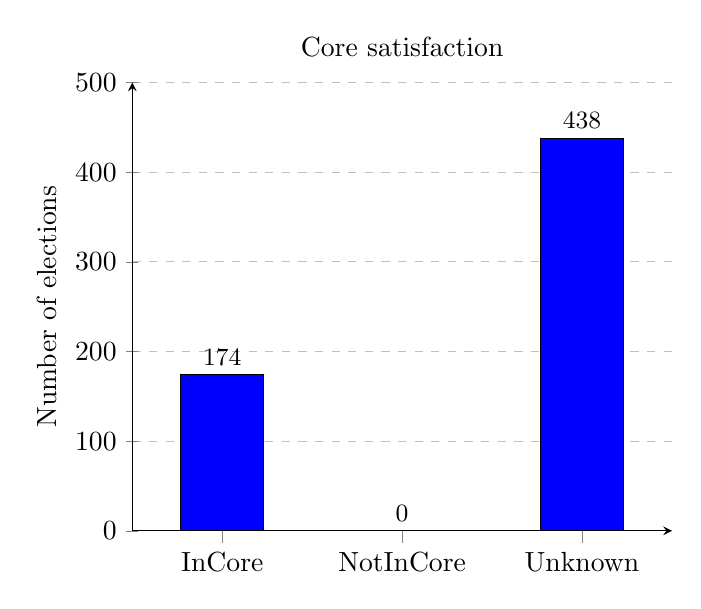
\begin{tikzpicture}
        \begin{axis}[
            axis lines=left,
            ybar,
            bar width=30pt,
            enlarge x limits=0.25,
            ylabel={Number of elections},
            ymin=0,
            ymax=500,
            xtick=data,
            xticklabels={InCore, NotInCore, Unknown},
            title={Core satisfaction},
            ymajorgrids=true,
            grid style=dashed,
            nodes near coords,
            every node near coord/.append style={font=\small},
        ]
        \addplot+[black, fill=blue] coordinates {(0,174) (1,0) (2,438)};
        \end{axis}
    \end{tikzpicture}
    \end{minipage}
    \begin{minipage}[c]{0.5\textwidth}
    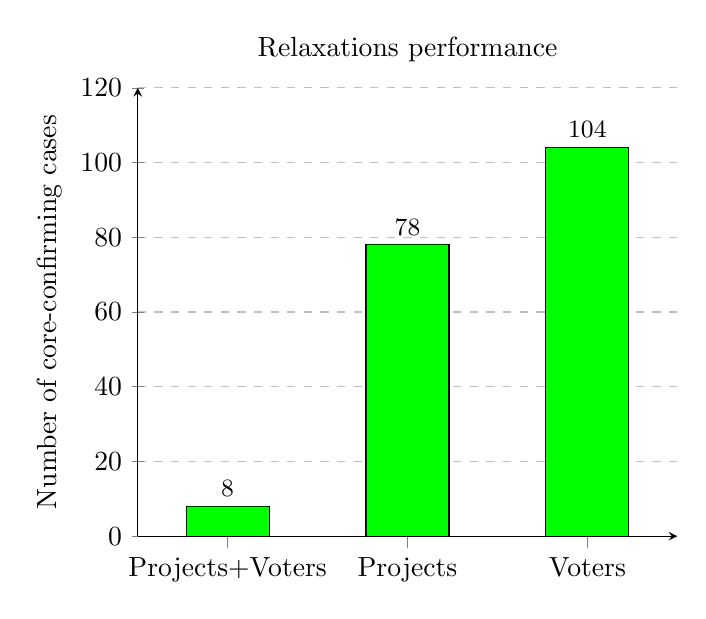
\begin{tikzpicture}
        \begin{axis}[
            axis lines=left,
            ybar,
            bar width=30pt,
            enlarge x limits=0.25,
            ylabel={Number of core-confirming cases},
            ymin=0,
            ymax=120,
            xtick=data,
            xticklabels={Projects+Voters, Projects, Voters},
            title={Relaxations performance},
            ymajorgrids=true,
            grid style=dashed,
            nodes near coords,
            every node near coord/.append style={font=\small},
        ]
        \addplot+[black, fill=green] coordinates {(0,8) (1,78) (2,104)};
        \end{axis}
    \end{tikzpicture}
    \end{minipage}
    \caption{
        Left: number of elections where the core status was determined using relaxations.
        Right: contribution of each relaxation method to the 174 elections confirmed to be in the core.
    }
    \label{relaxations-mes}
\end{figure}

Turning to Utilitarian Greedy, we observe an increase in runtime for the largest instances. Unlike MES, many UG outcomes do not satisfy the core. In such cases, after running each relaxation, we additionally execute the vanilla solver on the subset of projects and voters identified as potentially blocking by the relaxation. These additional times are not reflected in the charts, as they are insignificant. Among the 433 instances where core violation could not be confirmed initially, the relaxation method successfully identified blocking coalitions in 108 cases --- all of which were found using fractional solutions of the voters-relaxation LP. However, 325 instances remained unresolved.

\begin{figure}[h!]
    \centering
    \includegraphics[width=\chartsize\linewidth]{outputs/Relaxations/greedy.png}
    \caption{Combined execution times of core-verifying ILP with projects, voters, and both relaxations on Utilitarian Greedy outcomes.}
    \label{relaxations-greedy-time}
\end{figure}

\begin{figure}[h!]
    \begin{minipage}[c]{0.5\textwidth}
    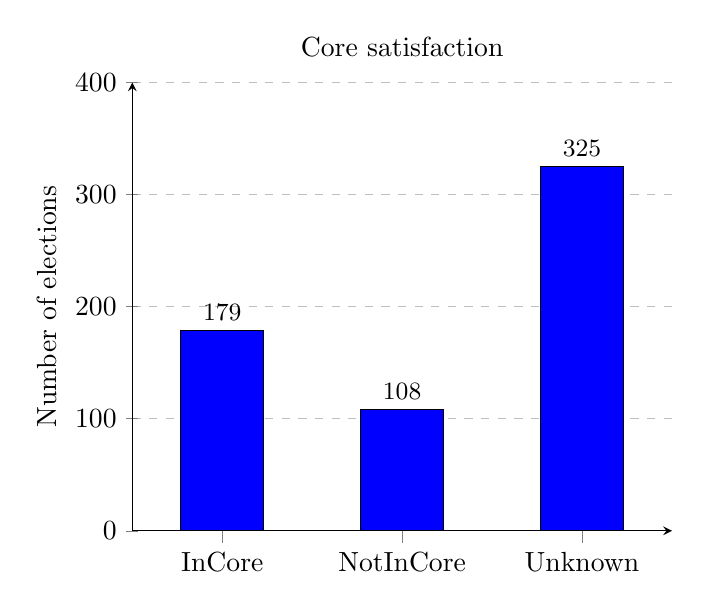
\begin{tikzpicture}
        \begin{axis}[
            axis lines=left,
            ybar,
            bar width=30pt,
            enlarge x limits=0.25,
            ylabel={Number of elections},
            ymin=0,
            ymax=400,
            xtick=data,
            xticklabels={InCore, NotInCore, Unknown},
            title={Core satisfaction},
            ymajorgrids=true,
            grid style=dashed,
            nodes near coords,
            every node near coord/.append style={font=\small},
        ]
        \addplot+[black, fill=blue] coordinates {(0,179) (1,108) (2,325)};
        \end{axis}
    \end{tikzpicture}
    \end{minipage}
    \begin{minipage}[c]{0.5\textwidth}
    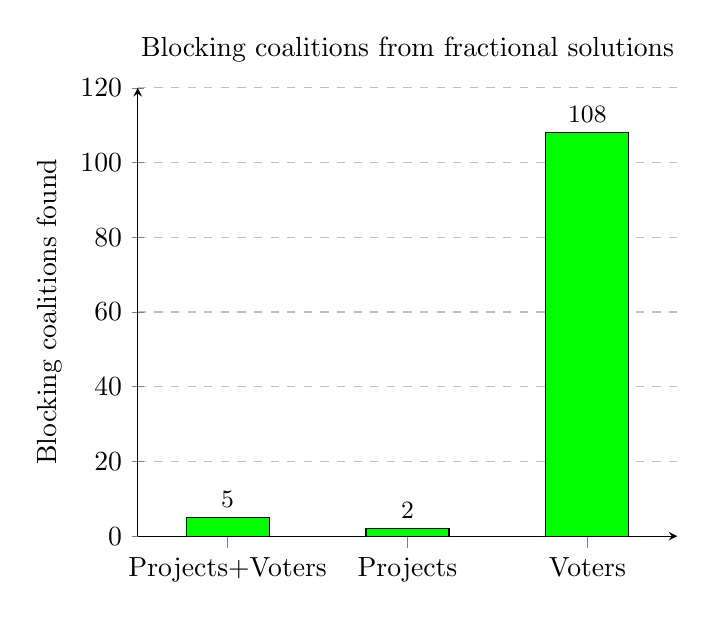
\begin{tikzpicture}
        \begin{axis}[
            axis lines=left,
            ybar,
            bar width=30pt,
            enlarge x limits=0.25,
            ylabel={Blocking coalitions found},
            ymin=0,
            ymax=120,
            xtick=data,
            xticklabels={Projects+Voters, Projects, Voters},
            title={Blocking coalitions from fractional solutions},
            ymajorgrids=true,
            grid style=dashed,
            nodes near coords,
            every node near coord/.append style={font=\small},
        ]
        \addplot+[black, fill=green] coordinates {(0,5) (1,2) (2,108)};
        \end{axis}
    \end{tikzpicture}
    \end{minipage}
    \caption{
        Left: number of elections where the core status was determined using relaxations.
        Right: number of elections where each relaxation found a blocking coalition from a fractional outcome.
    }
    \label{relaxations-greedy}
\end{figure}

\section{Branching Priority}

The \texttt{BranchPriority} attribute guides the solver's traversal of the branch-and-bound tree. Since outcomes from the Method of Equal Shares typically satisfy the core, the solver must explore the entire tree to confirm this. In such cases, this attribute, which aims to guide the solver toward feasible solutions more quickly, offers little to no benefit. However, runtimes for MES instances tend to be lower for medium-sized elections (see Figure~\ref{branching-priority-mes}).

\begin{figure}[h!]
    \centering
    \includegraphics[width=\chartsize\linewidth]{outputs/BranchingPriority/mes.png}
    \caption{Execution time of core-verifying ILP with Branching Priority heuristic on Method of Equal Shares outcomes.}
    \label{branching-priority-mes}
\end{figure}

For Utilitarian Greedy outcomes, it is worth noting that one instance in the \texttt{all\_50} dataset timed out (see Figure~\ref{branching-priority-greedy}). Interestingly, the execution time increased for UG outcomes when using the \texttt{BranchPriority} attribute. This may seem unintuitive at first. However, the likely explanation is that the solver is more effective at cutting subproblems when evaluating core-satisfying outcomes, where the most ,,important'' variables (according to the branching priority) play a main role. In contrast, blocking coalitions in UG outcomes often involve projects and voters with lower \texttt{BranchPriority} values, making branching less efficient in these cases.

\begin{figure}[h!]
    \centering
    \includegraphics[width=\chartsize\linewidth]{outputs/BranchingPriority/greedy.png}
    \caption{Execution time of core-verifying ILP with Branching Priority heuristic on Utilitarian Greedy outcomes.}
    \label{branching-priority-greedy}
\end{figure}

\section{Variable Start and Hint Values}

The next two variable attributes, \texttt{Start} and \texttt{VarHintVal}, serve a similar purpose to the previous one --- guiding the solver towards the most promising solution.

Performance decreases on MES outcomes for these attributes (see Figure~\ref{start-and-hint-mes}). The reason is that steering the solver toward a feasible solution is ineffective when no such solution exists, as in the case of core-satisfying outcomes.

\begin{figure}[h!]
    \centering
    \includegraphics[width=\chartsize\linewidth]{outputs/StartandVarHintVal/mes.png}
    \caption{Execution time of core-verifying ILP with Variable Start and Hint Values heuristic on Method of Equal Shares outcomes.}
    \label{start-and-hint-mes}
\end{figure}

In the UG case, we observe that the average execution time for the largest instances decreased by approximately one second --- a roughly 25\% improvement compared to the vanilla implementation. This suggests that our initial variable guesses are often correct, enabling the solver to identify blocking coalitions more effectively.

\begin{figure}[h!]
    \centering
    \includegraphics[width=\chartsize\linewidth]{outputs/StartandVarHintVal/greedy.png}
    \caption{Execution time of core-verifying ILP with Variable Start and Hint Values heuristic on Utilitarian Greedy outcomes.}
    \label{start-and-hint-greedy}
\end{figure}

\section{Removing maximal satisfied voters}

Removing voters who have already reached their maximum satisfaction can significantly reduce the size of the problem. While removing just a few percent of voters may not result in a noticeable performance boost, excluding over 90\%, which happens in some cases, can make a real difference.

For MES, one instance still timed out; however, 85\% of elections were solved in under a minute, compared to only 80\% in vanilla algorithm. The overall runtime significantly decreased, confirming the validity and potential of this approach.

\begin{figure}[h!]
    \centering
    \includegraphics[width=\chartsize\linewidth]{outputs/VotersRemoval/mes.png}
    \caption{Execution time of core-verifying ILP on Method of Equal Shares outcomes after removing maximal satisfied voters.}
    \label{voters-removal-mes}
\end{figure}

In the UG case, we also observe a slight performance improvement. While the speed-up is not as significant as in the previous section (approximately 17\% for the largest instances), it is still noticeable. As expected, smaller instances tend to be computed faster, which explains why this strategy yields benefits across both MES and UG outcomes.

\begin{figure}[h!]
    \centering
    \includegraphics[width=\chartsize\linewidth]{outputs/VotersRemoval/greedy.png}
    \caption{Execution time of core-verifying ILP on Utilitarian Greedy outcomes after removing maximal satisfied voters.}
    \label{voters-removal-greedy}
\end{figure}

\section{Essential Projects}

In the first section of this chapter, we observed that the Pareto optimality ILP, in its basic form, is already very fast. One might argue that no further improvements are necessary; however, this thesis explores one such enhancement, referred to as the essential projects optimization.

Similarly to the removal of maximal satisfied voters in the core verification program, the inclusion of essential projects here aims to reduce the search space and improve solver performance. As demonstrated in Figures~\ref{essential-projects-mes} and~\ref{essential-projects-greedy}, this optimization yields an approximate 10\% reduction in the average execution time for the MES outcomes. However, it has no significant impact on UG outcomes.

It is worth noting that Pareto optimality can already be verified by the basic algorithm in under 100 milliseconds for most instances, and execution times do not exceed 0.5 seconds for the largest ones. Therefore, although this optimization provides measurable improvements, further enhancements are generally unnecessary from a practical standpoint.

\begin{figure}[h!]
    \centering
    \includegraphics[width=\chartsize\linewidth]{outputs/EssentialProjects/mes.png}
    \caption{Execution time of PO-verifying ILP with Essential Projects heuristic on Method of Equal Shares outcomes.}
    \label{essential-projects-mes}
\end{figure}

\begin{figure}[h!]
    \centering
    \includegraphics[width=\chartsize\linewidth]{outputs/EssentialProjects/greedy.png}
    \caption{Execution time of PO-verifying ILP with Essential Projects heuristic on Utilitarian Greedy outcomes.}
    \label{essential-projects-greedy}
\end{figure}

\section{Combined Heuristics}

Let us now consider a combination of multiple heuristics in the core-verifying ILP. Specifically, we first remove maximally satisfied voters and then set the \texttt{BranchPriority}, \texttt{Start}, and \texttt{VarHintVal} variable attributes.

Starting with MES, we do not observe any improvements --- in fact, quite the opposite. The average runtime on \texttt{all\_50} instances doubles, and a significant number of the \texttt{all} instances results in timeouts (see Figure~\ref{combined-mes}). Once again, guiding the solver to find blocking coalitions in core-satisfying outcomes proves ineffective, as eventually the entire search space must be explored to verify core satisfaction.

\begin{figure}[h!]
    \centering
    \includegraphics[width=\chartsize\linewidth]{outputs/Combined/mes.png}
    \caption{Execution time of core-verifying ILP with all heuristics combined on Method of Equal Shares outcomes.}
    \label{combined-mes}
\end{figure}

For UG outcomes, on the other hand, we observe significant improvements on the largest instances --- the average runtime dropped from approximately 4.5 seconds to 2 seconds, resulting in an over 50\% speed-up (see Figure~\ref{combined-greedy}). However, execution times for other instance groups slightly increase, and one instance from the \texttt{all\_50} set results in a timeout. This might be due to the use of the \texttt{BranchPriority} attribute, as this heuristic was the only one that previously caused a timeout on this particular instance.

\begin{figure}[h!]
    \centering
    \includegraphics[width=\chartsize\linewidth]{outputs/Combined/greedy.png}
    \caption{Execution time of core-verifying ILP with all heuristics combined on Utilitarian Greedy outcomes.}
    \label{combined-greedy}
\end{figure}

\chapter{Algorithms Applications}
\label{algorithms-applications}

This chapter explores how various voting rules perform with respect to satisfying core and Pareto efficiency properties. Although many voting rules are known to satisfy Pareto optimality, an overview of which can be found in the recent work of Lackner and Skowron~\cite{20}, the core remains a more elusive and computationally challenging property. The following sections analyse specific voting rules and their empirical behaviour with respect to these two central metrics.

\section{Greedy Utilitarian Welfare}

As mentioned earlier, this rule aims to maximize the total utility of voters, which makes it a natural candidate for achieving Pareto optimality. Because Pareto efficiency is fundamentally about not being able to improve anyone’s outcome without making someone else worse off, maximizing aggregate utility tends to align well with this concept.

The experimental results, summarized in Figure~\ref{greedy-metrics}, show that the Greedy Utilitarian Welfare rule indeed satisfies Pareto optimality in all tested cases. However, this rule frequently violates the core. Since it focuses solely on overall utility and not on proportional fairness, it may neglect small but cohesive groups of voters. These groups could potentially form blocking coalitions by proposing alternative project sets that better represent their preferences and fall within their share of the budget.

Therefore, while Greedy Utilitarian Welfare is efficient in terms of utility, it is not well-suited for ensuring fairness or stability as captured by the core.

\begin{figure}[h!]
    \centering
    \includegraphics[width=0.46\linewidth]{outputs/MetricSatisfaction/greedy.png}
    \caption{Metrics satisfaction for Greedy Utilitarian Welfare.}
    \label{greedy-metrics}
\end{figure}

\section{Method of Equal Shares}

Equal Shares is widely recognized as a strong approximation to the core. Peters and Skowron~\cite{9} demonstrated that Equal Shares satisfies the core approximately, up to a logarithmic factor. This theoretical result makes it a good choice when seeking fairness and stability.

Empirical evaluation supports this perspective. As shown in Figure~\ref{mes-metrics}, Equal Shares produces outcomes that satisfy the core in all, but three cases --- Appendix~\ref{appendix:A} contains a deep analysis of one of the instances. This confirms its robustness in maintaining group fairness, even when the exact core membership is hard to compute. On the downside, Equal Shares does not perform as well in terms of Pareto efficiency even with the budget increment. This is expected as the method prioritizes proportional budget allocations and fairness over the maximization of total utility.

\begin{figure}[h!]
    \centering
    \includegraphics[width=0.46\linewidth]{outputs/MetricSatisfaction/mes.png}
    \caption{Metrics satisfaction for Method of Equal Shares.}
    \label{mes-metrics}
\end{figure}

Throughout this thesis, MES with budget increment (MES-Add1) was investigated. For the purpose of applications, Utilitarian Greedy completion for MES-Add1 was also benchmarked. With this enhancement, the rule always returns exhaustive outcomes, and it is harder to find a dominant set of projects, what is a trivial problem, with non-exhaustive ones. In result, all outcomes now satisfy Pareto optimality (see Figure~\ref{mes-ug-metrics}).

\begin{figure}[h!]
    \centering
    \includegraphics[width=0.46\linewidth]{outputs/MetricSatisfaction/mes-ug.png}
    \caption{Metrics satisfaction for MES-Add1U --- Method of Equal Shares with budget increment and Utilitarian Greedy completion.}
    \label{mes-ug-metrics}
\end{figure}

In conclusion, Equal Shares is a strong candidate for scenarios where fairness is a primary concern. One downside is non-exhaustive outcomes, but it is easy to be overcome with Utilitarian Greedy completion.

\section{Bounded Overspending}

Bounded Overspending, as a variant of the Method of Equal Shares, is expected to give results similar to MES.

Benchmarks indeed confirm this expectation. As shown in Figure~\ref{bos-metrics}, vast majority of outcomes satisfy the core, and all but two satisfy Pareto optimality. Overall, the results are slightly worse than those of MES with UG completion, but they remain strong -- clearly outperforming random allocations.

\begin{figure}[h!]
    \centering
    \includegraphics[width=0.46\linewidth]{outputs/MetricSatisfaction/bos.png}
    \caption{Metrics satisfaction for Bounded Overspending.}
    \label{bos-metrics}
\end{figure}

\section{Random Outcomes}

In contrast to other rules, the random selection of projects has been evaluated, with results presented in Figure~\ref{random-metrics}. Although this rule lacks strategic reasoning, its outcomes satisfy the core property in slightly more than half of the election instances from the Pabulib dataset. More surprisingly, in almost all cases, the returned outcome is also Pareto optimal. This result is notably better than that of the Method of Equal Shares and is comparable to the performance of the Utilitarian Greedy rule.

It is also worth noting the significant performance advantage of this approach. While computing the UG outcome takes a few seconds and MES may require even over a minute for larger instances, the random rule delivers results instantly. Despite its simplicity, it performs unexpectedly well with respect to our metrics.

\begin{figure}[h!]
    \centering
    \includegraphics[width=0.46\linewidth]{outputs/MetricSatisfaction/random.png}
    \caption{Metrics satisfaction for Random Rule.}
    \label{random-metrics}
\end{figure}

\chapter{Summary}
\label{summary}

The motivation for this thesis was to verify NP-hard properties as efficiently as possible, in order to evaluate various voting rules with respect to the core and other fairness criteria. For this purpose, linear programs were formulated for two key properties and then further optimized. All necessary models and voting rules had already been implemented in Pabutools, so integer linear programming became the main focus of this work.

The main goal of this thesis has been achieved --- we are able to verify the satisfaction of NP-hard properties, such as core and Pareto optimality, within finite (and reasonably small) computation time. While the latter can be computed very quickly, the former is significantly more challenging. Finding a blocking coalition is much easier than verifying that none exists. As a result, outcomes that satisfy the core property for large instances are more difficult to compute in a reasonable time.

To address this, a variety of improvement techniques have been explored and implemented, with most being successful. Several of these reduce the search space, enabling faster solutions, even for instances that previously led to timeouts. Core verification, in particular, became less complex in computation with these enhancements. Notable improvements include the use of the \texttt{BranchPriority} attribute, which significantly accelerated MES outcomes, as well as the \texttt{Start} and \texttt{VarHintVal} attributes, which improved the finding of blocking coalitions in UG outcomes. Also, combining the above attributes resulted in the most visible improvement for finding blocking coalitions in the largest instances. Additionally, removing voters who had already reached maximal satisfaction helped reduce the complexity of the search tree. Although the ILP formulation for Pareto optimality was already efficient, it was further improved by identifying and including essential projects.

Despite these performance improvements, some limitations remain. One of them is the existence of election instances for which MES outcomes could not be verified for core satisfaction within 30 minutes. In some cases, it took about half an hour and these times did not improve despite enhancements to the solver. This is strongly dependent on the structure of the election --- in particular, large instances without any blocking coalitions tend to require traversal of the entire, complex search space. A second limitation is that many of the implemented improvements are solver-specific and may not be portable to other solvers. However, the ILP formulations themselves can be rewritten for use with other high-performance optimizers and remain a valuable basis for future research.

Another major success is the effectiveness of the heuristics. The Method of Equal Shares proves to be a strong candidate for generating core allocations, while Utilitarian Greedy consistently yields Pareto optimal outcomes. Although MES by itself is not exhaustive, complementing it with UG produces a voting rule that is Pareto optimal and almost always produces core outcomes. Bounded Overspending, as a variation of MES, gives similar results. However, UG does not stand out as much compared to random exhaustive allocations in the context of these two properties.

Performance experiments using the Gurobi Optimizer also demonstrated its capabilities. The solver handles NP-hard properties exceptionally well --- in some cases, verifying fairness properties was faster than computing the election outcomes themselves. This underlines Gurobi's value and explains its widespread adoption in academic and industrial applications. Moreover, the optimizer can be further enhanced with additional variable attributes and hints beyond those discussed in this thesis, making it a highly practical tool.

Finally, this thesis serves as a proof of concept for applying linear programming techniques to computationally hard problems in the social choice theory. It opens new avenues for research on voting rules and demonstrates how integer linear programming can be leveraged to analyse complex metrics in realistic settings. One possible application within Pabustas could be to incorporate core and Pareto optimality checks as benchmarks of fairness, allowing users to evaluate how often different voting rules satisfy these particular properties.

In conclusion, this thesis demonstrates that even NP-hard problems, which are unsolvable for straightforward algorithms, can often be solved within seconds when reformulated as integer linear programs. This highlights the significant potential of the ILP technique for addressing other computationally hard problems, even beyond the domain of social choice theory.

\appendix

\chapter{An election instance where MES fails the core}
\label{appendix:A}

This appendix presents a small election instance from subunit Wawer, Warsaw 2018, where the Method of Equal Shares fails to return a core outcome.

\textbf{Setup:}
The election has a budget limit of $b=125{,}794$ and $|N|=301$ voters. There are five candidate projects with the following costs:
$$
\begin{array}{ll}
    \text{Project} & \text{Cost} \\
    \hline
    p_1 & 35{,}000 \\
    p_2 & 60{,}984 \\
    p_3 & 75{,}476 \\
    p_4 & 63{,}500 \\
    p_5 & 14{,}100
\end{array}
$$

\textbf{Voter preferences:}
The ballots are as follows:
$$
\begin{array}{cl|cl}
    \text{Group} & \text{Ballots} & \text{Group} & \text{Ballots} \\
    \hline
    G_1 & 8\times\{p_1, p_2, p_5\} & G_8 & 2\times\{p_3, p_5\} \\
    G_2 & 44\times\{p_1, p_3, p_5\} & G_9 & 2\times\{p_4, p_5\} \\
    G_3 & 2\times\{p_1, p_4, p_5\} & G_{10} & 2\times\{p_1\} \\
    G_4 & 2\times\{p_1, p_2\} & G_{11} & 6\times\{p_2\} \\
    G_5 & 9\times\{p_1, p_3\} & G_{12} & 6\times\{p_3\} \\
    G_6 & 191\times\{p_2, p_4\} & G_{13} & 7\times\{p_4\} \\
    G_7 & 1\times\{p_2, p_5\} & G_{14} & 19\times\{p_5\}
\end{array}
$$

\textbf{MES outcome and core violation:}  
MES returns the outcome $W=\{p_2,p_5\}$. However, this outcome is blocked by a coalition $S$ of 202 voters who prefer the alternative $T=\{p_4\}$ --- a violation of the core. Note that even if we artificially complete $W$ with project $p_1$ (which would make $W$ exhaustive), the same blocking coalition still applies.

\textbf{MES Execution Details:}  
In the first iteration, MES selects the most approved affordable project. Both $p_2$ and $p_4$ are strong candidates, but $p_2$ wins with 208 approvals (compared to 202 for $p_4$). Each of these 208 voters pays:
$$
\frac{cost(p_2)}{208}=\frac{60{,}984}{208}\approx293.38
$$

Given the per-voter budget of $b_i=b/|N|\approx417.92$, this leaves:
$$
b_i'=417.92-293.38\approx124.54
$$

The remaining budgets, grouped by the 14 voter ballot types listed above, are summarized below:
$$
\begin{array}{cc|cc}
    \text{Group} & \text{Remaining Budget} & \text{Group} & \text{Remaining Budget} \\
    \hline
    G_1 & 124.73 & G_8 & 417.92 \\
    G_2 & 417.92 & G_9 & 417.92 \\
    G_3 & 417.92 & G_{10} & 417.92 \\
    G_4 & 124.73 & G_{11} & 124.73 \\
    G_5 & 417.92 & G_{12} & 417.92 \\
    G_6 & 124.73 & G_{13} & 417.92 \\
    G_7 & 124.73 & G_{14} & 417.92
\end{array}
$$

The total remaining budget across all voters is 64,810.

In the second iteration, MES evaluates which projects can be afforded using only the remaining budgets of their supporters:
$$
\begin{tabular}{c|c}
    Project & Supporters' Total Budget \\
    \hline
    $p_1$ & 25{,}068.74 \\
    $p_3$ & 25{,}493.12 \\
    $p_4$ & 28{,}420.55 \\
    $p_5$ & 30{,}252.24
\end{tabular}
$$

Only $p_5$ is affordable at this stage, so it is added in the second (and final) iteration.

\textbf{Completion with Greedy Rule:}  
The remaining budget after MES is 50,710. When applying Utilitarian Greedy completion, the only affordable project is $p_1$, which is then added. However, as noted earlier, the final outcome $\{p_2,p_5,p_1\}$ still fails the core property.

\begin{thebibliography}{99}
\addcontentsline{toc}{chapter}{Bibliography}

\bibitem{1} S. Rey, G. Pierczyński, M. Utke, and P. Skowron. \textit{Pabutools}
\url{https://pypi.org/project/pabutools/}

\bibitem{2} \textit{Pabulib}.
\url{https://pabulib.org/}

\bibitem{3} \textit{Pabustats}.
\url{https://pabulib.org/wsgi/analysis/menu}

\bibitem{4} B. Fain, A. Goel, and K. Munagala. The Core of the Participatory Budgeting Problem.
\textit{Lecture Notes in Computer Science}, pages 384--399, 2016.
doi: 10.1007/978-3-662-54110-4\_27.

\bibitem{5} H. Aziz, J. Lang, and J. Monnot. Computing and testing Pareto optimal committees.
2018.
doi: 10.48550/arXiv.1803.06644.

\bibitem{6} Gurobi Optimization, LLC. \textit{Gurobi}.
\url{https://www.gurobi.com/}

\bibitem{7} G. Nowakowski. \textit{Linear Programs source code}.
\url{https://github.com/COMSOC-Community/pabutools/pull/52}

\bibitem{8} G. Nowakowski. \textit{Analysis source code}.
\url{https://github.com/grzenow4/Masters-Thesis}

\bibitem{9} D. Peters and P. Skowron. Proportionality and the limits of welfarism.
In \textit{Proceedings of the 2020 ACM Conference on Economics and Computation}, pages 793--794, 2020.
doi: 10.1145/3391403.3399465. Extended version arXiv:1911.11747.

\bibitem{10} D. Peters and P. Skowron. \textit{Method of Equal Shares website}.
\url{https://equalshares.net/}

\bibitem{11} G. Papasotiropoulos, S. Z. Pishbin, O. Skibski, P. Skowron, and T. Wąs. Method of Equal Shares with Bounded Overspending.
2024.
doi: 10.48550/arXiv.2409.15005.

\bibitem{12} H. Aziz, M. Brill, V. Conitzer, E. Elkind, R. Freeman, and T. Walsh. Justified representation in approval-based committee voting.
\textit{Social Choice and Welfare}, 48(2):461--485, 2017.
doi: 10.1007/s00355-016-1019-3.

\bibitem{13} K. Munagala, Y. Shen, and K. Wang. Auditing for Core Stability in Participatory Budgeting.
\textit{Lecture Notes in Computer Science}, pages 292--310, 2022.
doi: 0.1007/978-3-031-22832-2\_17.

\bibitem{14} K. Munagala, Y. Shen, K. Wang, and Z. Wang. Approximate Core for Committee Selection via Multilinear Extension and Market Clearing.
In \textit{Proceedings of the 33rd ACM-SIAM Symposium on Discrete Algorithms (SODA-2022)}, pages 2229--2252, 2022.
doi: 10.1137/1.9781611977073.89.

\bibitem{15} M. Brill, P. Gölz, D. Peters, U. Schmidt-Kraepelin, and K. Wilker. Approval-based apportionment.
\textit{Mathematical Programming}, 2022.
doi: 10.1007/s10107-022-01852-1.

\bibitem{16} M. Lackner and P. Skowron. Multi-Winner Voting with Approval Preferences.
2023.
doi: 10.1007/978-3-031-09016-5.

\bibitem{17} D. Peters, G. Pierczyński, and P. Skowron. Proportional participatory budgeting with additive utilities.
In \textit{Proceedings of the Thirty-fifth Conference on Neural Information Processing Systems (NeurIPS-2021)}, pages 12726--12737, 2021.
doi: 10.48550/arXiv.2008.13276.

\bibitem{18} M. Lackner and P. Skowron. Utilitarian welfare and representation guarantees of approval-based multiwinner rules.
2020.
doi: 10.1016/j.artint.2020.103366.

\bibitem{19} G. B. Dantzig. \textit{Simplex Method}.
\url{https://en.wikipedia.org/wiki/Simplex_algorithm}

\bibitem{20} M. Lackner and P. Skowron. Consistent approval-based multi-winner rules.
Technical Report
arXiv:1704.02453v1 [cs.GT], arXiv.org, 2017.

\end{thebibliography}

\end{document}

%%% Local Variables:
%%% mode: latex
%%% TeX-master: t
%%% coding: latin-2
%%% End:
